%%%%%%%%%%%%%%%%%%%%%%%%%%%%%%%%%%%%%%%%%
% Lachaise Assignment
% LaTeX Template
% Version 1.0 (26/6/2018)
%
% This template originates from:
% http://www.LaTeXTemplates.com
%
% Authors:
% Marion Lachaise & François Févotte
% Vel (vel@LaTeXTemplates.com)
%
% License:
% CC BY-NC-SA 3.0 (http://creativecommons.org/licenses/by-nc-sa/3.0/)
% 
%%%%%%%%%%%%%%%%%%%%%%%%%%%%%%%%%%%%%%%%%

%----------------------------------------------------------------------------------------
%	PACKAGES AND OTHER DOCUMENT CONFIGURATIONS
%----------------------------------------------------------------------------------------

\documentclass{article}

%%%%%%%%%%%%%%%%%%%%%%%%%%%%%%%%%%%%%%%%%
% Lachaise Assignment
% Structure Specification File
% Version 1.0 (26/6/2018)
%
% This template originates from:
% http://www.LaTeXTemplates.com
%
% Authors:
% Marion Lachaise & François Févotte
% Vel (vel@LaTeXTemplates.com)
%
% License:
% CC BY-NC-SA 3.0 (http://creativecommons.org/licenses/by-nc-sa/3.0/)
% 
%%%%%%%%%%%%%%%%%%%%%%%%%%%%%%%%%%%%%%%%%

%----------------------------------------------------------------------------------------
%	PACKAGES AND OTHER DOCUMENT CONFIGURATIONS
%----------------------------------------------------------------------------------------
\usepackage{listings}
\usepackage{amsmath,amsfonts,stmaryrd,amssymb} % Math packages
\usepackage{amsthm}

\usepackage{enumerate} % Custom item numbers for enumerations

\usepackage[linesnumbered,ruled,vlined]{algorithm2e} % Algorithms

\usepackage[framemethod=tikz]{mdframed} % Allows defining custom boxed/framed environments
\usepackage{subfigure}
\usepackage{listings} % File listings, with syntax highlighting
\usepackage{booktabs}
\usepackage{diagbox}

\lstset{
	basicstyle=\ttfamily, % Typeset listings in monospace font
}

%----------------------------------------------------------------------------------------
%	DOCUMENT MARGINS
%----------------------------------------------------------------------------------------

\usepackage{geometry} % Required for adjusting page dimensions and margins

\geometry{
	paper=a4paper, % Paper size, change to letterpaper for US letter size
	top=2.5cm, % Top margin
	bottom=3cm, % Bottom margin
	left=2.5cm, % Left margin
	right=2.5cm, % Right margin
	headheight=14pt, % Header height
	footskip=1.5cm, % Space from the bottom margin to the baseline of the footer
	headsep=1.2cm, % Space from the top margin to the baseline of the header
	%showframe, % Uncomment to show how the type block is set on the page
}

%----------------------------------------------------------------------------------------
%	FONTS
%----------------------------------------------------------------------------------------

\usepackage[utf8]{inputenc} % Required for inputting international characters
\usepackage[T1]{fontenc} % Output font encoding for international characters
% \usepackage{XCharter} % Use the XCharter fonts
\usepackage{CTEX}
\usepackage[hidelinks]{hyperref}

%----------------------------------------------------------------------------------------
%	COMMAND LINE ENVIRONMENT
%----------------------------------------------------------------------------------------

% Usage:
% \begin{commandline}
%	\begin{verbatim}
%		$ ls
%		
%		Applications	Desktop	...
%	\end{verbatim}
% \end{commandline}

\mdfdefinestyle{commandline}{
	leftmargin=10pt,
	rightmargin=10pt,
	innerleftmargin=15pt,
	middlelinecolor=black!50!white,
	middlelinewidth=2pt,
	frametitlerule=false,
	backgroundcolor=black!5!white,
	frametitle={Command Line},
	frametitlefont={\normalfont\sffamily\color{white}\hspace{-1em}},
	frametitlebackgroundcolor=black!50!white,
	nobreak,
}

% Define a custom environment for command-line snapshots
\newenvironment{commandline}{
	\medskip
	\begin{mdframed}[style=commandline]
}{
	\end{mdframed}
	\medskip
}

%----------------------------------------------------------------------------------------
%	FILE CONTENTS ENVIRONMENT
%----------------------------------------------------------------------------------------

% Usage:
% \begin{file}[optional filename, defaults to "File"]
%	File contents, for example, with a listings environment
% \end{file}

\mdfdefinestyle{file}{
	innertopmargin=1.6\baselineskip,
	innerbottommargin=0.8\baselineskip,
	topline=false, bottomline=false,
	leftline=false, rightline=false,
	leftmargin=2cm,
	rightmargin=2cm,
	singleextra={%
		\draw[fill=black!10!white](P)++(0,-1.2em)rectangle(P-|O);
		\node[anchor=north west]
		at(P-|O){\ttfamily\mdfilename};
		%
		\def\l{3em}
		\draw(O-|P)++(-\l,0)--++(\l,\l)--(P)--(P-|O)--(O)--cycle;
		\draw(O-|P)++(-\l,0)--++(0,\l)--++(\l,0);
	},
	nobreak,
}

% Define a custom environment for file contents
\newenvironment{file}[1][File]{ % Set the default filename to "File"
	\medskip
	\newcommand{\mdfilename}{#1}
	\begin{mdframed}[style=file]
}{
	\end{mdframed}
	\medskip
}

%----------------------------------------------------------------------------------------
%	NUMBERED QUESTIONS ENVIRONMENT
%----------------------------------------------------------------------------------------

% Usage:
% \begin{question}[optional title]
%	Question contents
% \end{question}

\mdfdefinestyle{question}{
	innertopmargin=1.2\baselineskip,
	innerbottommargin=0.8\baselineskip,
	roundcorner=5pt,
	nobreak,
	singleextra={%
		\draw(P-|O)node[xshift=1em,anchor=west,fill=white,draw,rounded corners=5pt]{%
		Question \theQuestion\questionTitle};
	},
}

\newcounter{Question} % Stores the current question number that gets iterated with each new question

% Define a custom environment for numbered questions
\newenvironment{question}[1][\unskip]{
	\bigskip
	\stepcounter{Question}
	\newcommand{\questionTitle}{~#1}
	\begin{mdframed}[style=question]
}{
	\end{mdframed}
	\medskip
}

%----------------------------------------------------------------------------------------
%	WARNING TEXT ENVIRONMENT
%----------------------------------------------------------------------------------------

% Usage:
% \begin{warn}[optional title, defaults to "Warning:"]
%	Contents
% \end{warn}

\mdfdefinestyle{warning}{
	topline=false, bottomline=false,
	leftline=false, rightline=false,
	nobreak,
	singleextra={%
		\draw(P-|O)++(-0.5em,0)node(tmp1){};
		\draw(P-|O)++(0.5em,0)node(tmp2){};
		\fill[black,rotate around={45:(P-|O)}](tmp1)rectangle(tmp2);
		\node at(P-|O){\color{white}\scriptsize\bf !};
		\draw[very thick](P-|O)++(0,-1em)--(O);%--(O-|P);
	}
}

% Define a custom environment for warning text
\newenvironment{warn}[1][Warning:]{ % Set the default warning to "Warning:"
	\medskip
	\begin{mdframed}[style=warning]
		\noindent{\textbf{#1}}
}{
	\end{mdframed}
}

%----------------------------------------------------------------------------------------
%	INFORMATION ENVIRONMENT
%----------------------------------------------------------------------------------------

% Usage:
% \begin{info}[optional title, defaults to "Info:"]
% 	contents
% 	\end{info}

\mdfdefinestyle{info}{%
	topline=false, bottomline=false,
	leftline=false, rightline=false,
	nobreak,
	singleextra={%
		\fill[black](P-|O)circle[radius=0.4em];
		\node at(P-|O){\color{white}\scriptsize\bf i};
		\draw[very thick](P-|O)++(0,-0.8em)--(O);%--(O-|P);
	}
}

% Define a custom environment for information
\newenvironment{info}[1][Info:]{ % Set the default title to "Info:"
	\medskip
	\begin{mdframed}[style=info]
		\noindent{\textbf{#1}}
}{
	\end{mdframed}
}
 % Include the file specifying the document structure and custom commands

%----------------------------------------------------------------------------------------
%	ASSIGNMENT INFORMATION
%----------------------------------------------------------------------------------------

\title{基于L-BFGS方法的神经网络训练} % Title of the assignment

\author{pangbo} % Author name and email address

\date{\today} % University, school and/or department name(s) and a date

%----------------------------------------------------------------------------------------

\begin{document}

\maketitle % Print the title


\section{背景} % Unnumbered section

在深度学习领域,绝大部分情况下会选择一阶优化方法进行神经网络模型参数优化,本文将尝试使用二阶拟牛顿类优化方法进行神经网络训练。通过与常见的神经网络优化方法进行对比,分析深度学习领域中二阶拟牛顿类优化方法的优势和劣势。

\subsection{全连接网络}

深度学习是机器学习的一个分支,它是一种基于神经网络的机器学习技术,用于模仿人脑的功能,支持从大量数据中进行预测和分类。神经网络本质上是一个有众多参数的复杂函数,训练的过程就是对这些参数进行调整,最终使其较好地拟合数据。

全连接网络是最简单的神经网络结构,它的每个神经元都与前一层的所有神经元相连,形成一个密集的连接结构。全连接网络的每个神经元都有一个权重向量和一个偏置项,输入向量限于权重向量进行内积,加上偏置项,再通过激活函数进行非线性变换,便可以得到神经元的输出。

单层全连接网络可以表示成如下的数学形式:
\begin{align*}
z^{(l)} = W^{(l)}a^{(l-1)} + b^{(l)}\\
a^{(l)} = f(z^{(l)})
\end{align*}

其中$a^{(l-1)}$是上一层神经元的输出,$W^{(l)}$是第$l$层的权重矩阵,$b^{(l)}$是偏置项,每一层的$W$、$b$的集合被称为这个神经网络的参数,$f$是激活函数,$a^{(l)}$是当前层神经元的输出。类比于生物神经元,$a$是神经元的轴突,用于输出信号,$W^{(l)}$代表了神经元之间的连接关系。

神经网络的训练过程,就是通过调整权重矩阵和偏置项,使得网络的输出尽可能地接近于真实值。为了衡量网络输出的误差,我们需要定义一个损失函数。损失函数会输出一个标量,这个标量代表了网络输出与真实值的差距。对于回归问题,常用的损失函数是均方误差,对于分类问题,常用的损失函数是交叉熵。

记损失函数为$L$,模型参数为$\theta$,样本输入为$x$,真实值为$y^*$,模型预测结果为$y=f(x;\theta)$。则神经网络的训练过程可以表示为如下的优化问题:
\begin{align*}
\min_{\theta} L(f(x;\theta), y^*)
\end{align*}
这是一个典型的无约束优化问题,优化目标为最小化损失函数。

对于一个线性全连接网络,无论有多少层,都可以用一个线性变换来表示。因此,为了能够表示更复杂的函数,我们需要引入非线性变换,即激活函数。常用的激活函数有sigmoid函数、tanh函数、ReLU函数等。这些激活函数的引入,使得神经网络可以表示更复杂的函数,从而提高了神经网络的表达能力。但同时,也使得整个网络所描述的变得复杂,难以从理论上快速找到其全局最优解。

\subsection{随机梯度下降}

梯度下降是一种一阶优化方法,基本思想是沿着梯度的反方向,以一定的步长进行迭代,直到达到收敛条件。梯度下降算法的迭代公式如下:
\begin{align*}
\theta_{t+1} = \theta_t - \eta \nabla L(\theta_t)
\end{align*}

损失函数值被看作一个关于模型参数的函数,通过求导找到最速下降方向,然后沿着这个方向进行参数更新。对于神经网络,使用线搜索确定步长的计算开销较大,因此一般使用较为固定的步长,即学习率$\eta$。

梯度下降算法的收敛性较好,但是每次迭代的计算开销较大,因为每次迭代都需要在整个训练集上计算梯度。在实际实现过程中,受限于内存容量,一般每次迭代只计算一个小批量样本的梯度,然后进行参数更新。这种算法被称为随机梯度下降算法,随机梯度下降及其变种是深度学习中最常用的优化算法。

\subsection{拟牛顿类算法}

牛顿法的基本思想是利用迭代点处的一阶导数(梯度)和二阶导数(Hessian矩阵)对目标函数进行二次函数近似,然后把二次模型的极小点作为新的迭代点,并不断重复这一过程,直至求得满足精度的近似极小值。牛顿法的迭代公式如下:
\begin{align*}
\theta_{t+1} = \theta_t - \eta [\nabla^2 L(\theta_t)]^{-1} \nabla L(\theta_t)
\end{align*}

牛顿法在选择下降路径时,能更好地拟合目标函数的局部曲面,在许多情况下,牛顿法能获得更快的收敛速度。但是牛顿法的计算开销较大,因为每次迭代都需要计算Hessian矩阵的逆矩阵。为了降低计算开销,人们提出了拟牛顿法,它通过近似Hessian矩阵的逆矩阵,来降低计算开销。BFGS公式是目前最有效的拟牛顿更新公式之一,它将Hessian矩阵的逆矩阵近似为一个对称正定矩阵,并限制每轮的更新的秩为2。

BFGS公式需要记录上一轮的拟牛顿矩阵,其大小与待优化参数的平方成正比,对于神经网络这种拥有大量参数的优化问题,保存拟牛顿矩阵的内存开销较大。为了降低内存开销,人们提出了L-BFGS算法,它只需要保存最近的$m$轮的梯度和更新步长,从而将内存开销降低到$O(md)$,其中$d$是参数的维度。

本文将尝试使用L-BFGS算法进行神经网络的训练。

\section{L-BFGS算法}

对于BFGS公式,其迭代形式可以表示为
\begin{align}
H_{k+1} = (V_k)^T H_k V_k + \rho_k s_k s_k^T
\label{bfgs-update}
\end{align}
其中
\begin{align*}
V_k &= I - \rho_k y_k s_k^T\\
\rho_k &= \frac{1}{y_k^T s_k}\\
y_k &= \nabla f(x_{k+1}) - \nabla f(x_k)\\
s_k &= x_{k+1} - x_k
\end{align*}

在公式\ref{bfgs-update}中,$H_k$是第$k$轮的拟牛顿矩阵,可以继续套用公式\ref{bfgs-update}获得,以此类推,L-BFGS算法无需保存拟牛顿矩阵,从而减少内存开销。

对于迭代$m$次的L-BFGS算法,$H_{k}$的计算过程如下:
\begin{equation}
\begin{aligned}
H_{k} 
=& V_{k-1}^TV_{k-2}^T\cdots V_{k-m}^TH_0V_{k-m}V_{k-m+1}\cdots V_{k-1}\\
&+V_{k-1}^TV_{k-2}^T\cdots V_{k-m+1}^T\rho_{k-m}s_{k-m}s_{k-m}^TV_{k-m+1}V_{k-m+2}\cdots V_{k-1}\\
&+V_{k-1}^TV_{k-2}^T\cdots V_{k-m+2}^T\rho_{k-m+1}s_{k-m+1}s_{k-m+1}^TV_{k-m+2}V_{k-m+3}\cdots V_{k-1}\\
&\quad\quad\cdots\cdots\\
&+V_{k-1}^T\rho_{k-2}s_{k-2}s_{k-2}^TV_{k-1}\\
&+\rho_{k-1}s_{k-1}s_{k-1}^T
\label{bfgs-iter-m}
\end{aligned}
\end{equation}

公式\ref*{bfgs-iter-m}在实际实现中,$V$矩阵是一个$d\times d$矩阵,这意味着计算过程中依然有大量的内存开销峰值,此外公式\ref*{bfgs-iter-m}涉及大量重复的矩阵乘法,计算开销也较大。

在实际的L-BFGS算法实现中,常使用两次循环递推进行计算,其伪代码见算法\ref{alg:two-loop}。

\begin{center}
	\begin{minipage}{0.75\linewidth} 

    \begin{algorithm}[H]
    \label{alg:two-loop}
    \DontPrintSemicolon
    \KwIn{Gradient $g_k$, Scaling factor $\gamma_k$, History size $m$, Past gradients $\{s_{k-i}, y_{k-i}\}_{i=1}^m$}
    \KwOut{Search direction $d_k$}
    \SetKwProg{Fn}{Function}{:}{}
    \SetKwFunction{FRecurs}{TwoLoopRecursion}\Fn{\FRecurs{$g_k$, $\gamma_k$, $\{s_{k-i}, y_{k-i}\}_{i=1}^m$}}{
        $q \leftarrow g_k$\;
        \For{$i = k-1 \to k-m$}{
            $\alpha_i \leftarrow \frac{s_i^\top q}{y_i^\top s_i}$\;
            $q \leftarrow q - \alpha_i y_i$\;
        }
        $r \leftarrow \gamma_k q$\;
        \For{$i = k-m \to k-1$}{
            $\beta \leftarrow \frac{y_i^\top r}{y_i^\top s_i}$\;
            $r \leftarrow r + s_i (\alpha_i - \beta)$\;
        }
        \KwRet{$-r$}\;
    }
    \caption{Two-loop recursion for L-BFGS}
    \end{algorithm}
	\end{minipage}
\end{center}

算法\ref{alg:two-loop}与公式\ref*{bfgs-iter-m}形式有较大差异,接下来我们将证明算法\ref{alg:two-loop}实现的正确性。

\begin{proof}
    首先考虑第一个循环,其递推形式为
    \begin{align*}
        \alpha_i &= \rho_is_i^Tq_{i+1}\\
        q_i &= q_{i+1} - \alpha_iy_i
    \end{align*}
    于是
    \begin{align*}
        q_{i}&=q_{i+1}-\alpha_iy_i\\
        &=(I-\rho_iy_is_i^T)q_{i+1}\\
        &=V_iq_{i+1}
    \end{align*}
    因为$q_{k}=\nabla f_k$,所以对于$i=k-1,k-2,\cdots,k-m$都有$q_i=V_{i}V_{i+1}\cdots V_{k-1}\nabla f_k$。

    再考虑第二个循环,其递推形式为
    \begin{align*}
        \beta_i &= \rho_iy_i^Tr_{i-1}\\
        r_{i} &= r_{i-1}+s_i(\alpha_i-\beta_i)
    \end{align*}
    于是
    \begin{align*}
        r_i &= r_{i-1}+s_i(\rho_is_i^Tq_{i+1}-\rho_iy_i^Tr_{i-1})\\
        &= (I-\rho_is_iy_i^T)r_{i-1}+\rho_is_is_i^Tq_{i+1}\\
        &= V_i^Tr_{i-1}+\rho_is_is_i^TV_{i+1}V_{i+2}\cdots V_{k-1}\nabla f_k
    \end{align*}

    展开递归,
    \begin{align*}
        r_i
        =& V_i^TV_{i-1}^Tr_{i-2}+V_i^T\rho_{i-1}s_{i-1}s_{i-1}^TV_{i}V_{i+1}\cdots V_{k-1}\nabla f_k+\rho_is_is_i^TV_{i+1}V_{i+2}\cdots V_{k-1}\nabla f_k\\
        =& V_i^TV_{i-1}^T\cdots V_{k-m}^Tr_{k-m-1}\\
        &+V_i^TV_{i-1}^T\cdots V_{k-m+1}^T\rho_{k-m}s_{k-m}s_{k-m}^TV_{k-m+1}V_{k-m+2}\cdots V_{k-1}\nabla f_k\\
        &+V_i^TV_{i-1}^T\cdots V_{k-m+2}^T\rho_{k-m+1}s_{k-m+1}s_{k-m+1}^TV_{k-m+2}V_{k-m+3}\cdots V_{k-1}\nabla f_k\\
        &\quad\quad\cdots\cdots\\
        &+V_i^T\rho_{i-1}s_{i-1}s_{i-1}^TV_{i}V_{i+1}\cdots V_{k-1}\nabla f_k\\
        &+\rho_is_is_i^TV_{i+1}V_{i+2}\cdots V_{k-1}\nabla f_k
    \end{align*}

    其中递归的初始值为
    \begin{align*}
        r_{k-m-1} = H_0q_{k-m} =H_0V_{k-m}V_{k-m+1}\cdots V_{k-1}\nabla f_k
    \end{align*}

    最终有
    \begin{align*}
        r_{k-1}
        =& V_{k-1}^TV_{k-2}^T\cdots V_{k-m}^TH_0V_{k-m}V_{k-m+1}\cdots V_{k-1}\nabla f_k\\
        &+V_{k-1}^TV_{k-2}^T\cdots V_{k-m+1}^T\rho_{k-m}s_{k-m}s_{k-m}^TV_{k-m+1}V_{k-m+2}\cdots V_{k-1}\nabla f_k\\
        &+V_{k-1}^TV_{k-2}^T\cdots V_{k-m+2}^T\rho_{k-m+1}s_{k-m+1}s_{k-m+1}^TV_{k-m+2}V_{k-m+3}\cdots V_{k-1}\nabla f_k\\
        &\quad\quad\cdots\cdots\\
        &+V_{k-1}^T\rho_{k-2}s_{k-2}s_{k-2}^TV_{k-1}\nabla f_k\\
        &+\rho_{k-1}s_{k-1}s_{k-1}^T\nabla f_k
    \end{align*}

    观察上式与公式\ref*{bfgs-iter-m}的形式,不难发现$r_{k-1}=H_k\nabla f_k$。也就是说$-r_{k-1}$就是我们要找的下降方向,算法\ref{alg:two-loop}是正确的。
\end{proof}

\section{实验}

\subsection{简单优化问题}

我们首先尝试使用L-BFGS算法求解两个经典的优化问题,分别为Rosenbrock函数和Rastrigin函数。

\begin{itemize}
    \item Rosenbrock函数
    $$
    f(x) = (a - x_0)^2 + b \cdot (x_1 - x_0^2)^2
    $$
    \item Rastrigin函数
    $$
    f(\mathbf{x}) = An + \sum_{i=1}^{n} \left[ x_i^2 - A \cos(2\pi x_i) \right]
    $$
\end{itemize}

这两个函数对于二维输入的函数图像如图\ref{fig:func_fig}所示,这是两个典型的非凸函数,能在一点程度上反映优化算法的性能。

我们使用L-BFGS算法与梯度下降求解这两个函数的最小值,优化结果如图\ref{fig:optimization_results}所示。可以看出,L-BFGS算法能够在较少的迭代次数内找到较好的解,而梯度下降算法难以在这样的非凸优化问题上获得一个收敛的结果。


\begin{figure}
    \centering
    \subfigure[Rosenbrock函数]{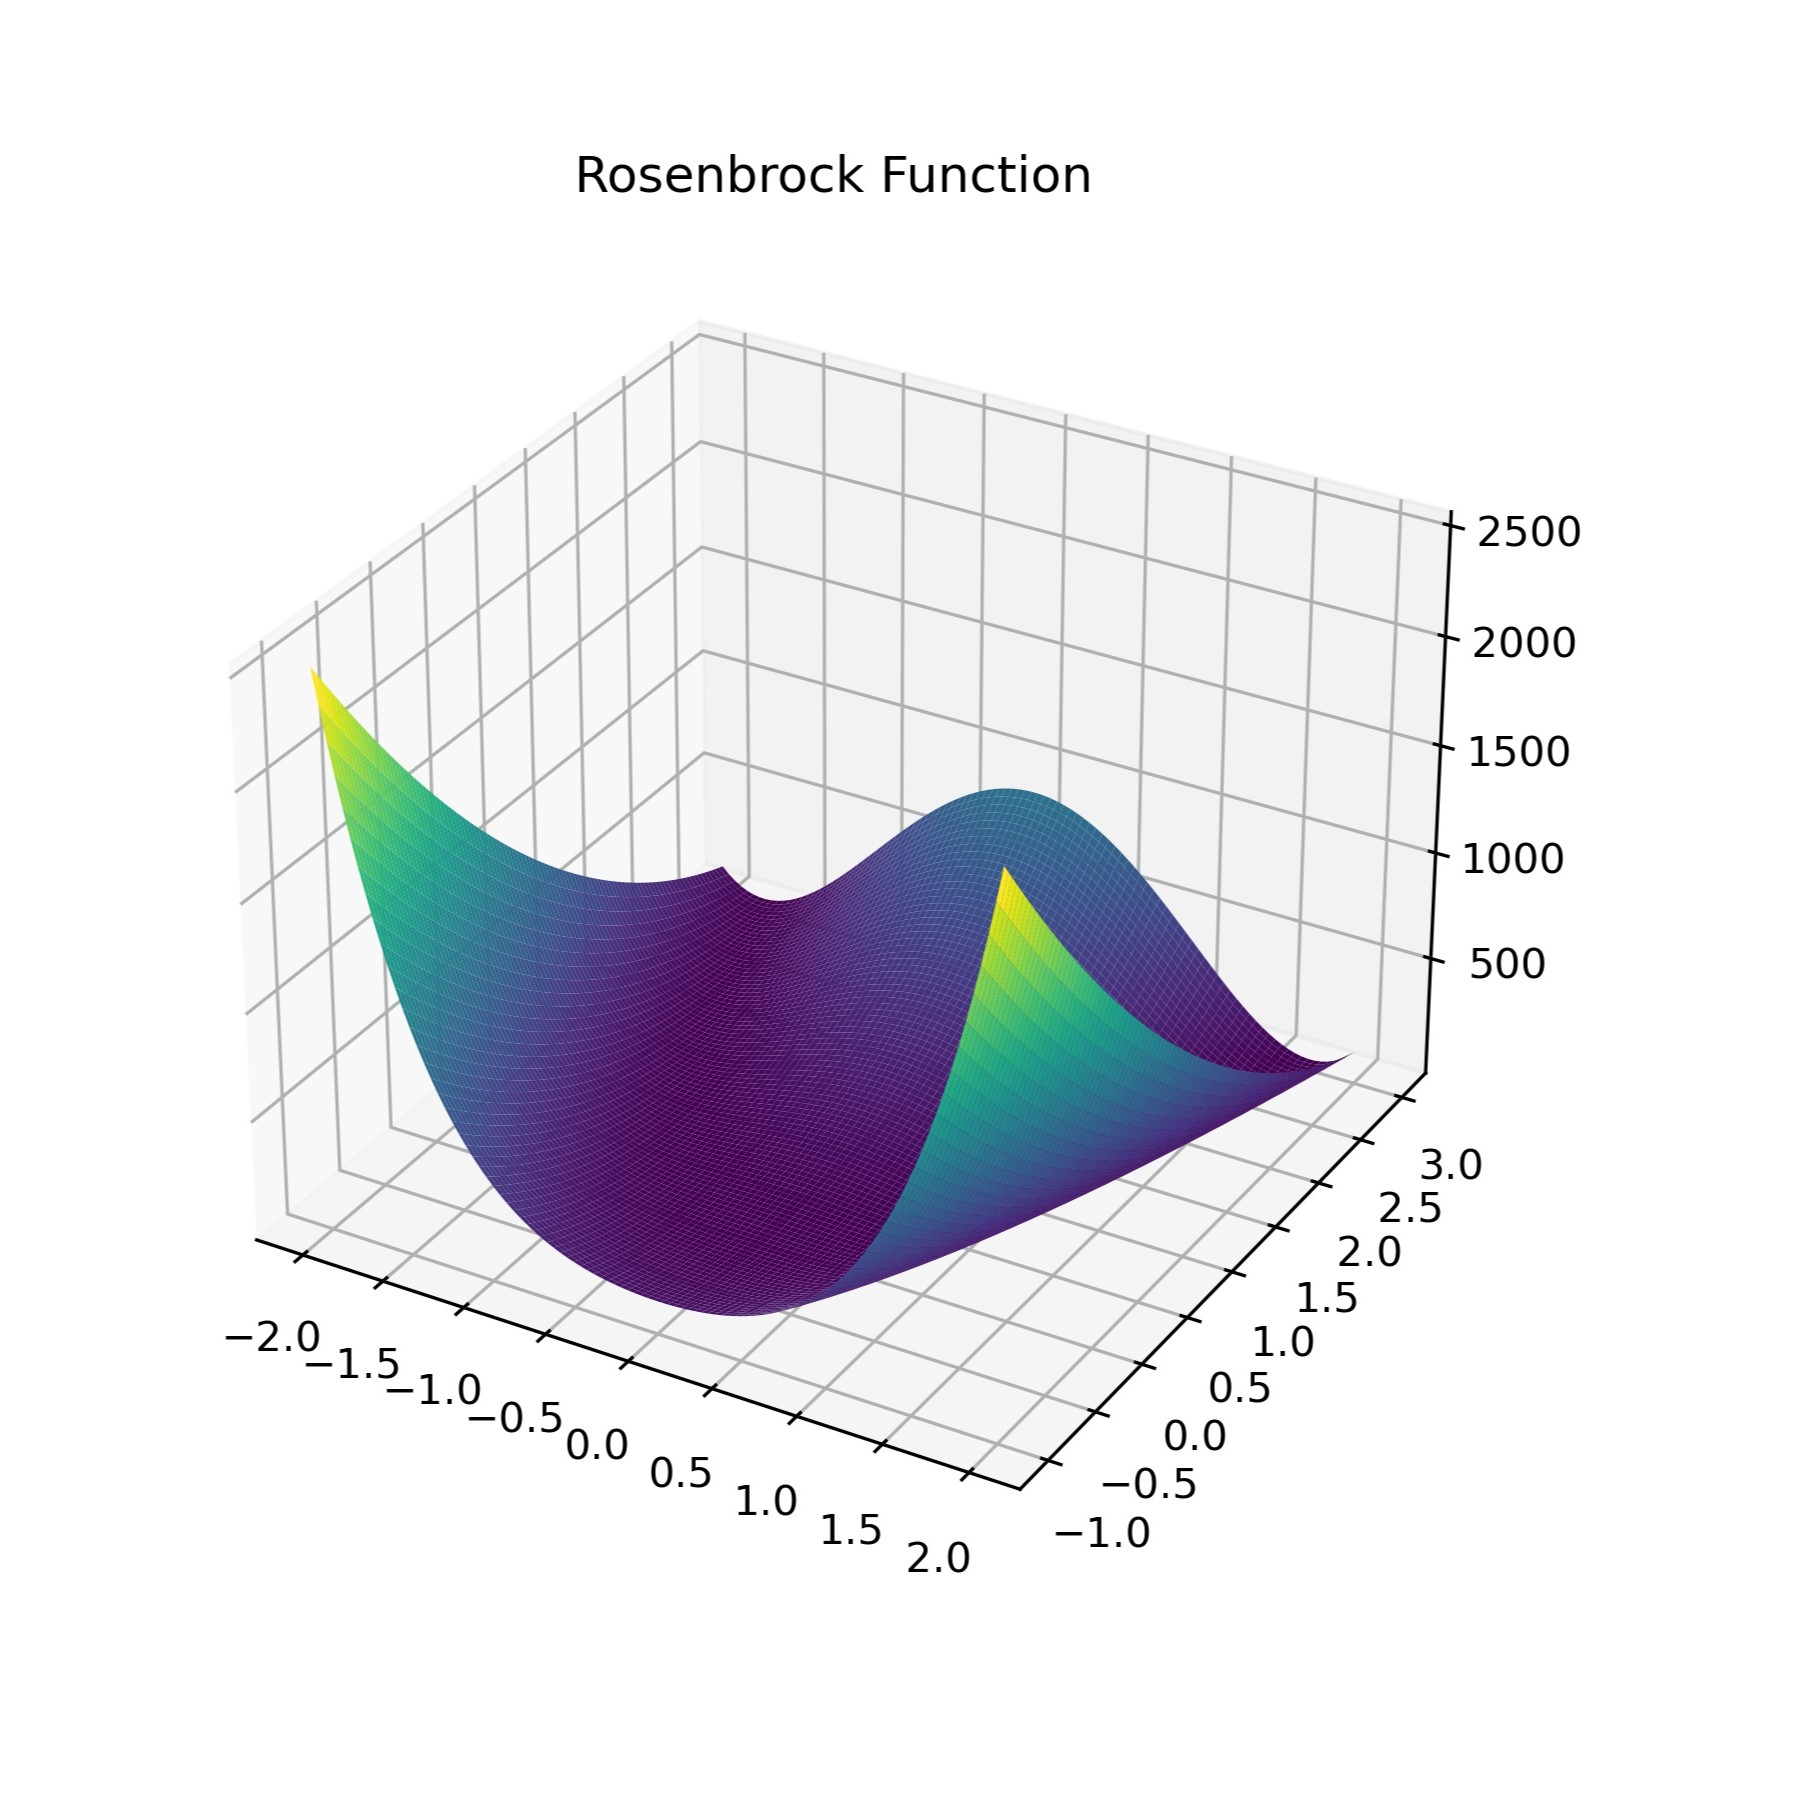
\includegraphics[width=0.45\linewidth]{fig-Rosenbrock-func.jpg}}
    \hspace{1cm}
    \subfigure[Rastrigin函数]{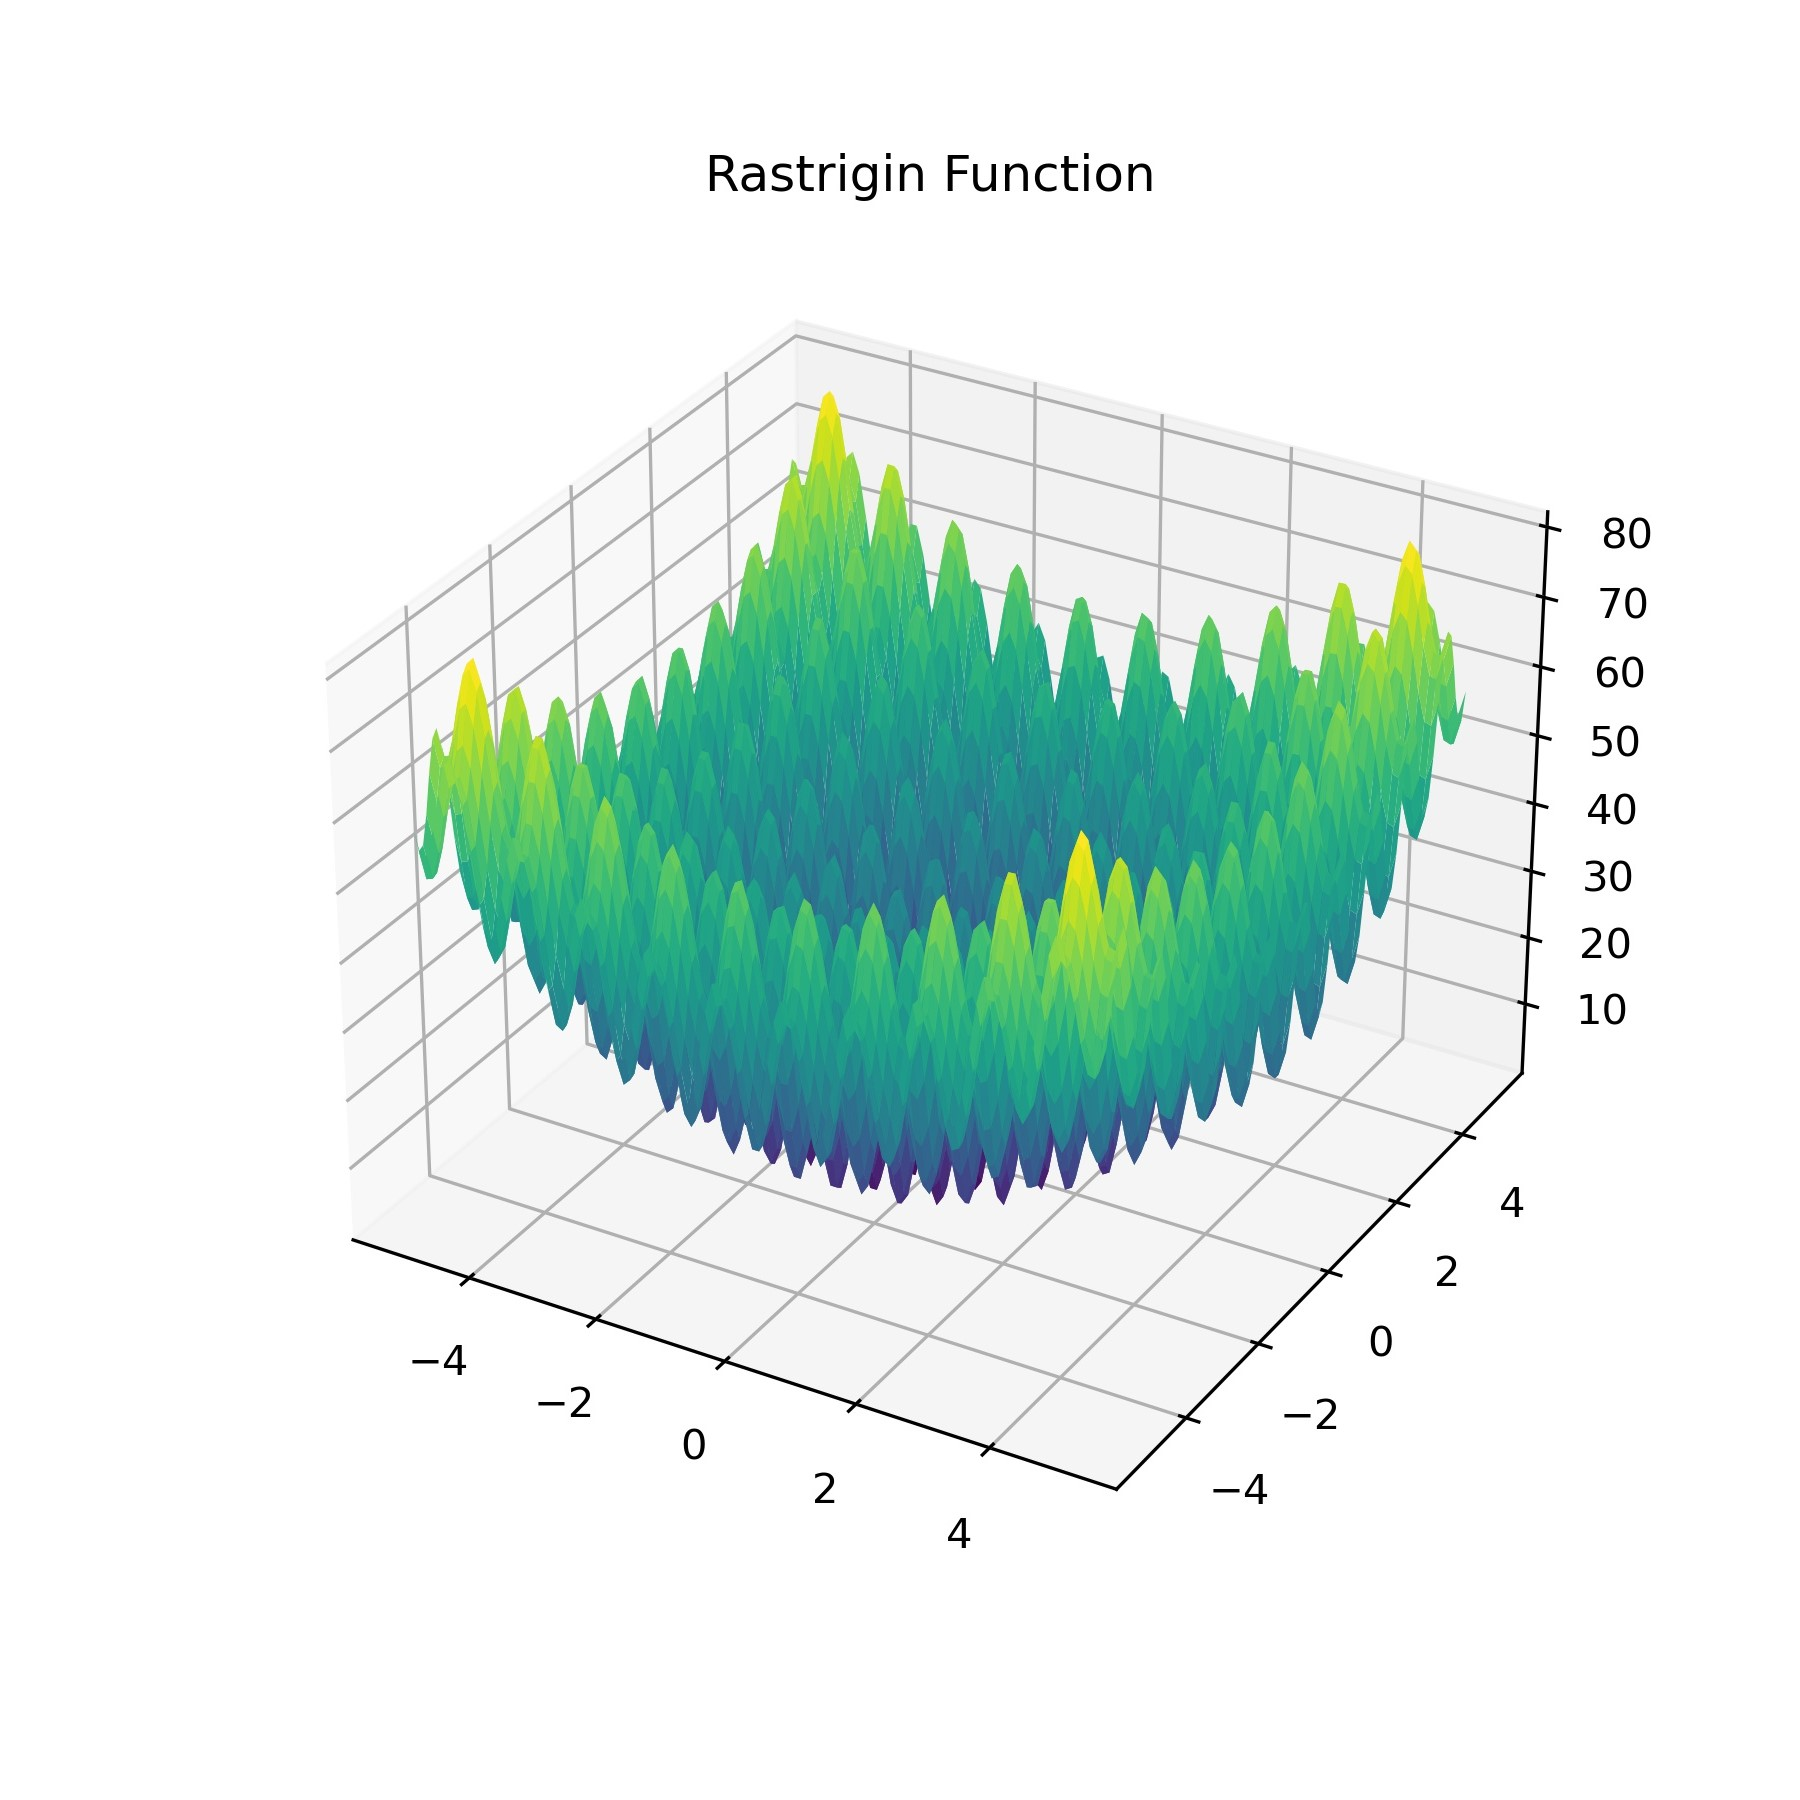
\includegraphics[width=0.45\linewidth]{fig-Rastrigin-func.jpg}}
    \caption{函数图像}
    \label{fig:func_fig}
\end{figure}

\begin{figure}
    \centering
    \subfigure[Rosenbrock函数]{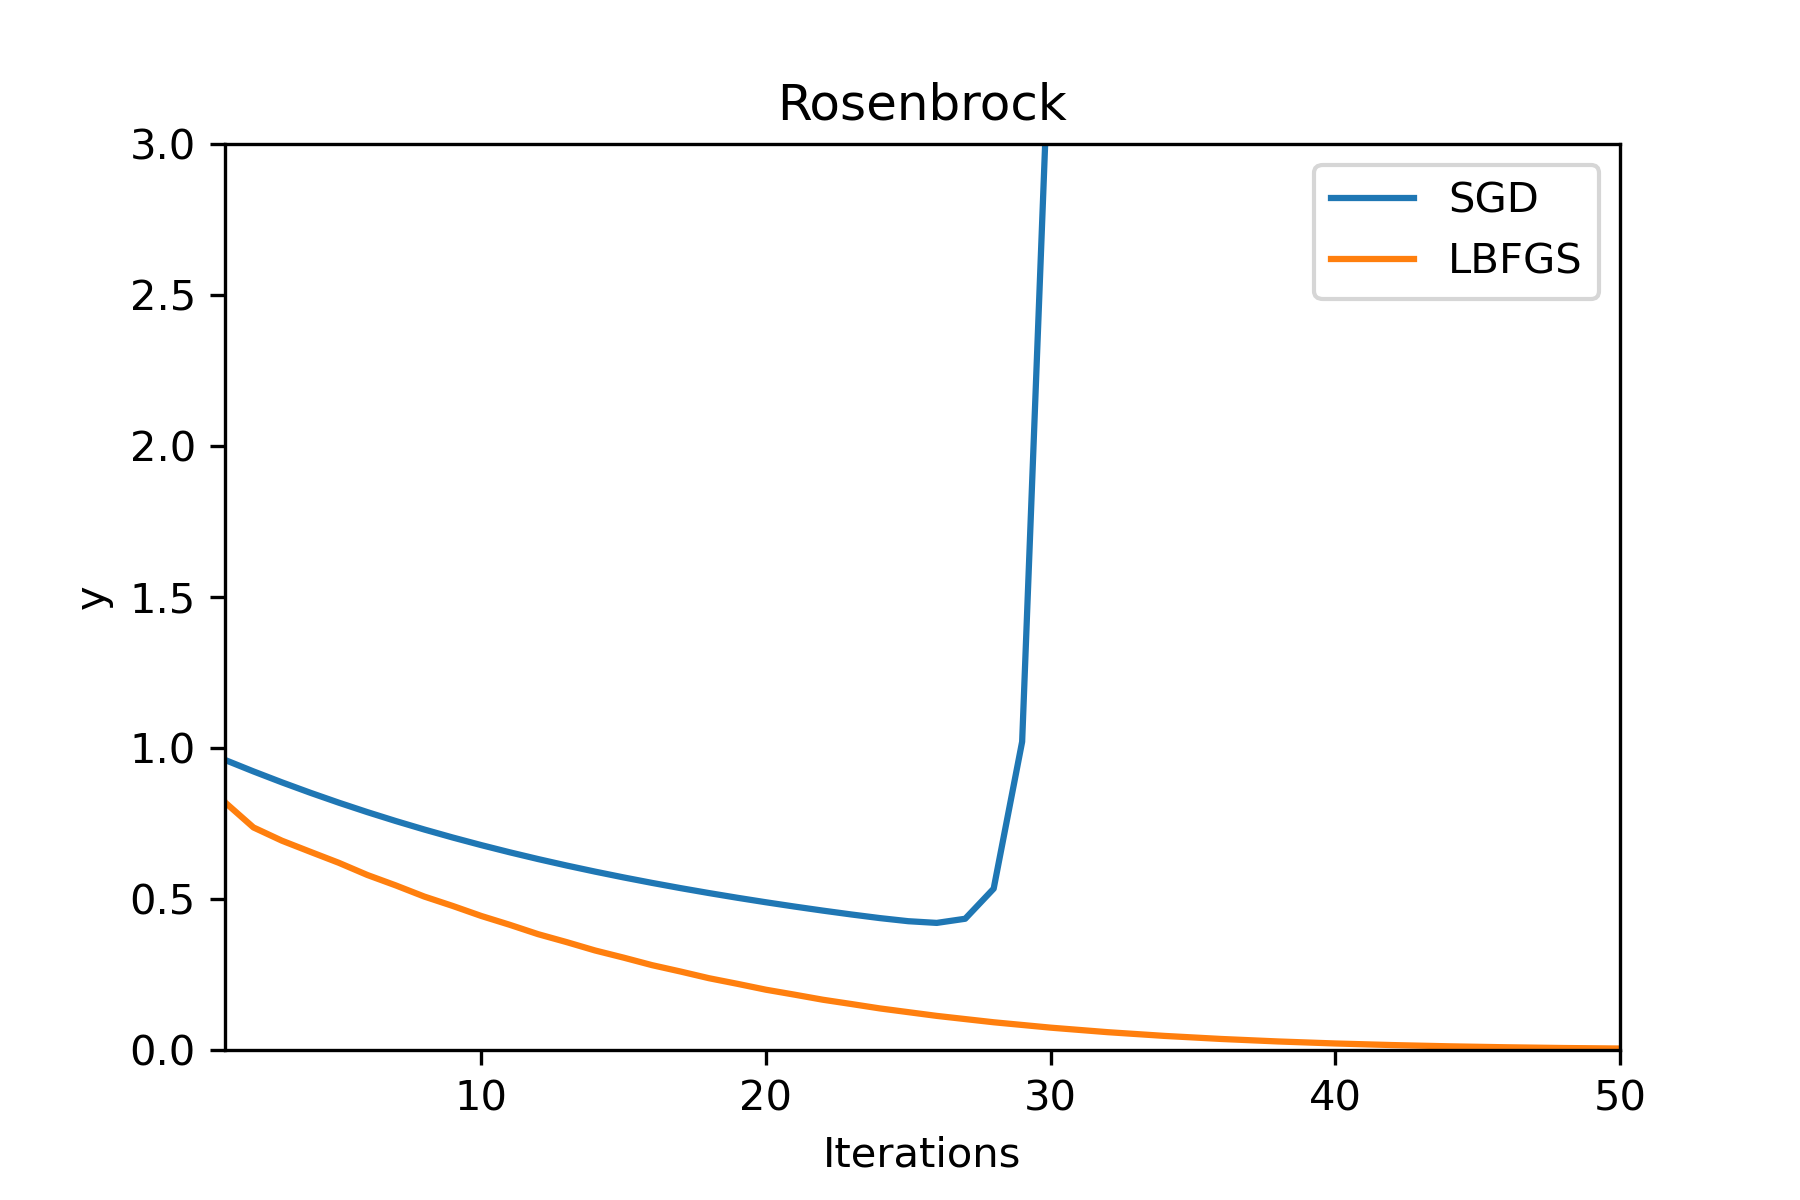
\includegraphics[width=0.45\linewidth]{fig-Rosenbrock-opt.png}}
    \hspace{1cm}
    \subfigure[Rastrigin函数]{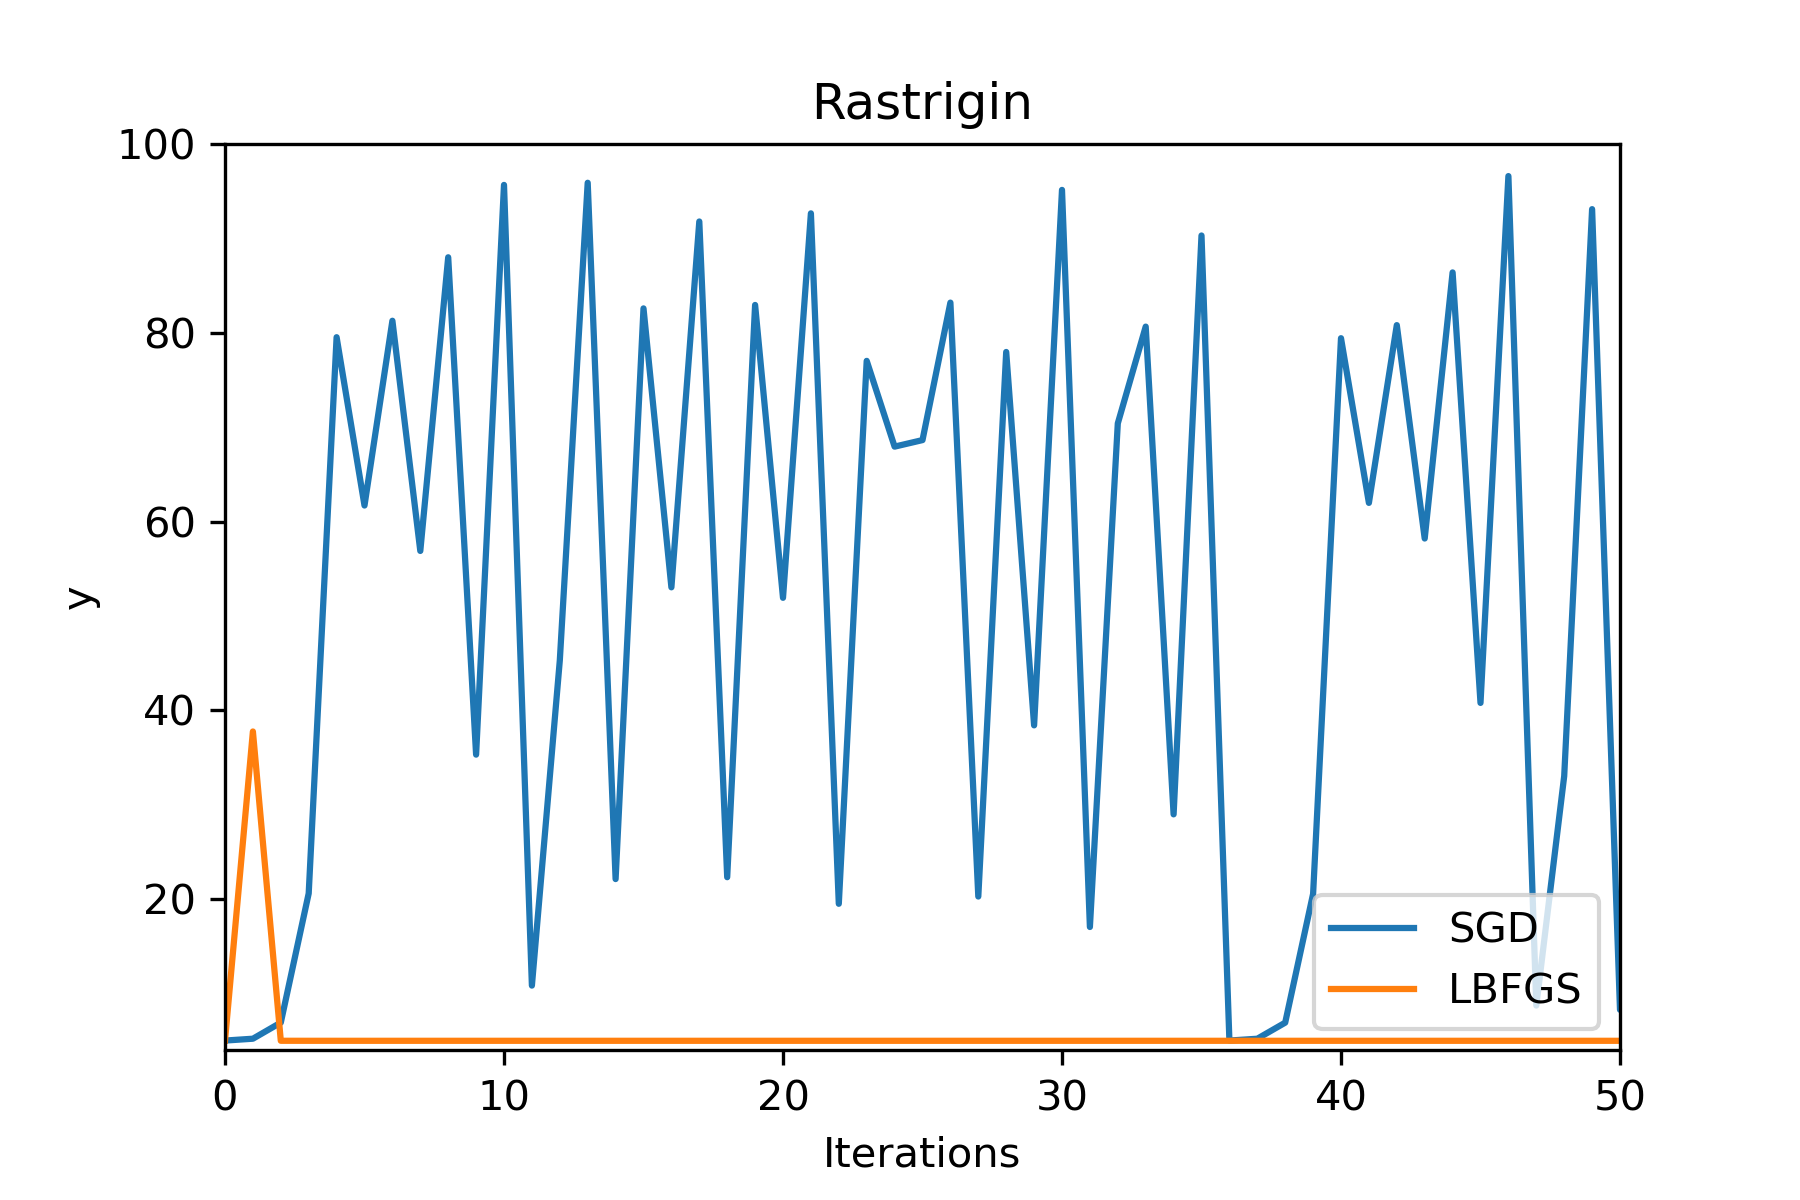
\includegraphics[width=0.45\linewidth]{fig-Rastrigin-opt.png}}
    \caption{优化结果}
    \label{fig:optimization_results}
\end{figure}

\subsection{神经网络训练}

我们选用手写数据集MNIST作为训练数据集,尝试使用多种优化算法对一个简单卷积神经网络进行训练。我们选用的三种优化方法分别为随机梯度下降、Adam算法和L-BFGS算法。其中随机梯度下降是一阶优化方法,Adam算法是一种基于梯度的一阶优化方法,在随机梯度下降的基础上,引入了动量项和二阶矩项,动态调节单次参数更新的步长,从而提高了训练速度。L-BFGS算法则为我们实现的拟牛顿方法。

首先,我们选择固定的样本进行训练,相比于真实的神经网络场景,这是一个简化的环境。真实的神经网络训练中,由于样本量较大,不能一次性放入模型计算,只能分批选出样本计算损失,这导致需要优化的目标是随时变化的,而不是固定的。在我们的简化环境中,我们只选择了少量样本,因此可以直接计算所有样本的损失,从而得到固定的优化目标。在固定样本上的训练结果如图\ref{fig:mnist_fix_train}所示,可以看到Adam算法的收敛速度最快,L-BFGS算法次之,随机梯度下降最慢。

\begin{figure}
    \centering
    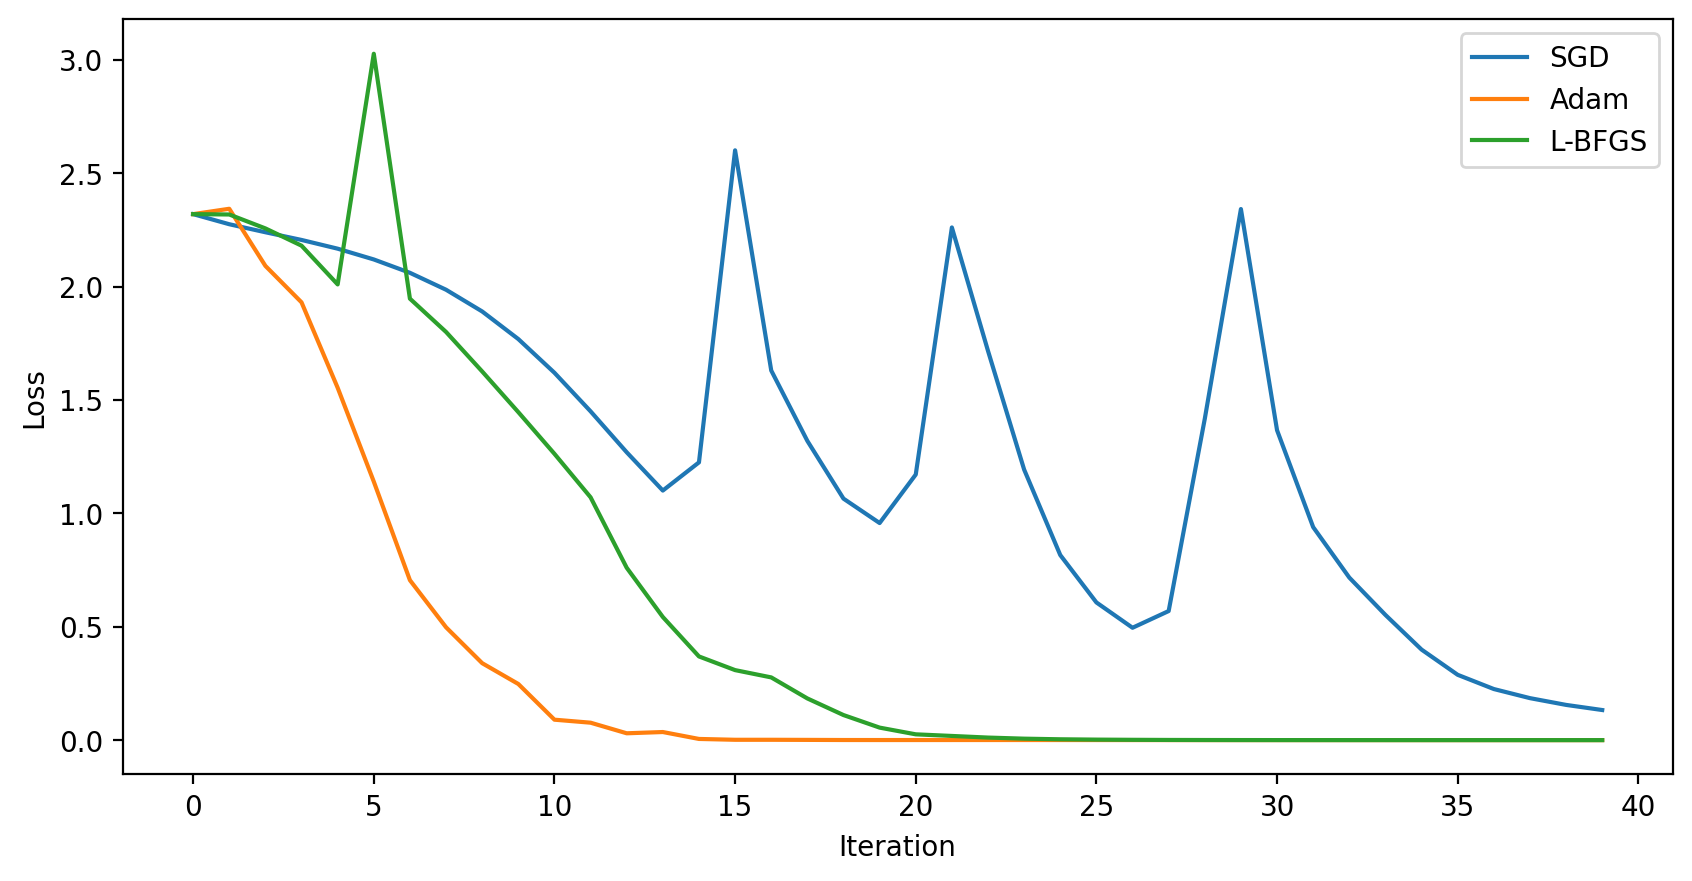
\includegraphics[width=0.8\linewidth]{fig-mnist-fix-train.png}
    \caption{固定样本的训练结果}
    \label{fig:mnist_fix_train}
\end{figure}

然后,我们在完整的MNIST数据集上训练,训练过程中的损失函数值如图\ref{fig:mnist_train}所示。

\begin{figure}
    \centering
    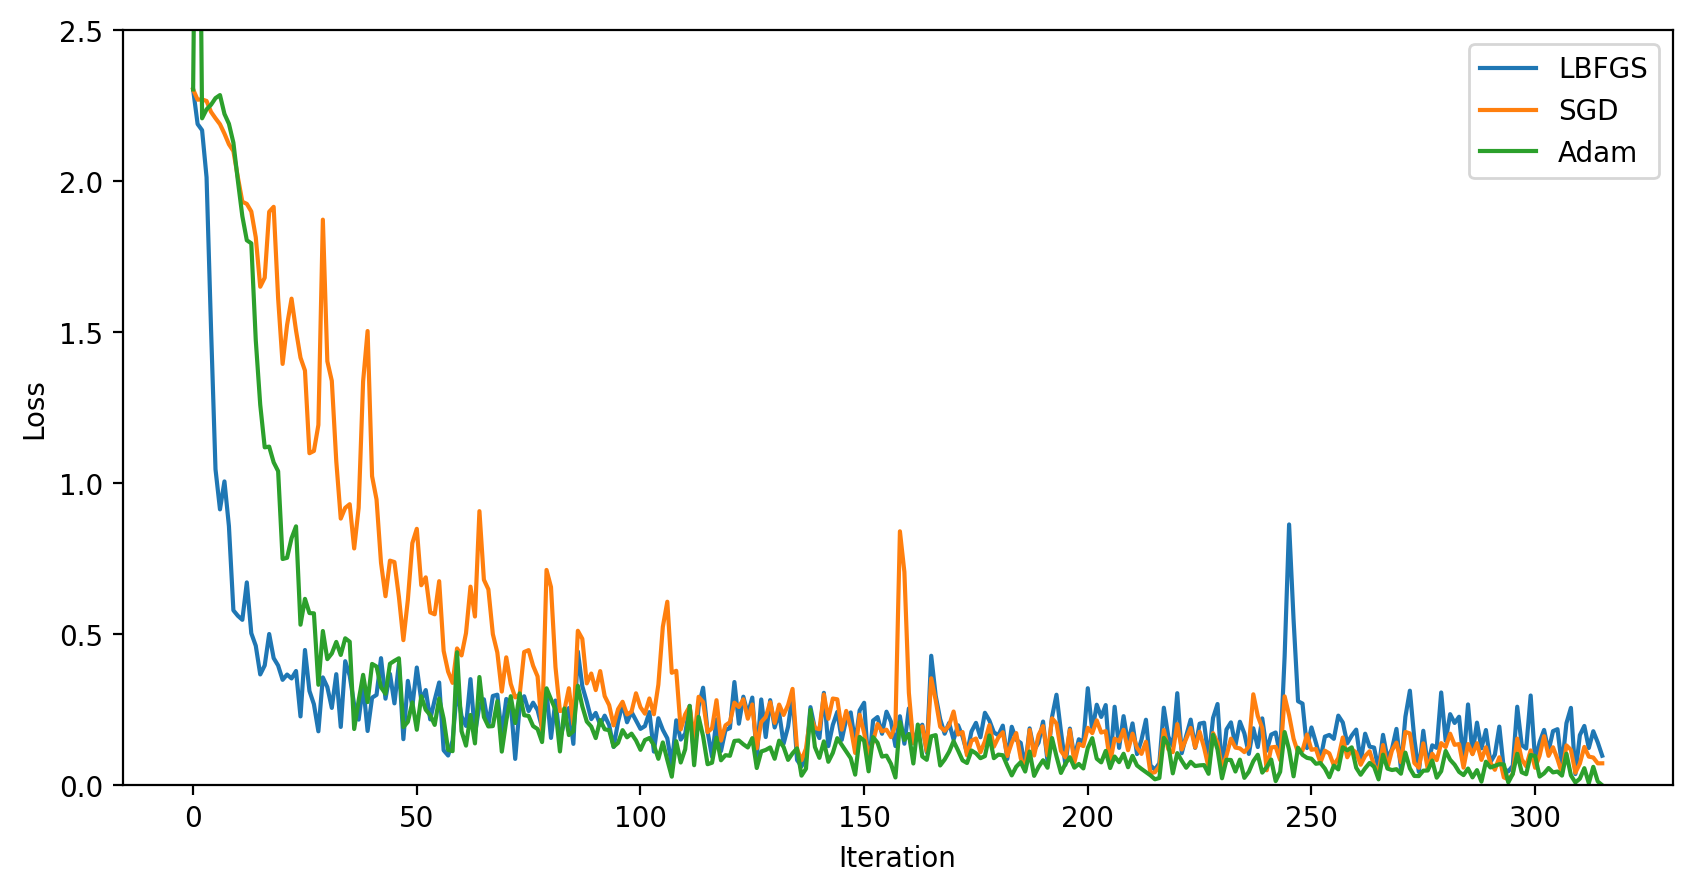
\includegraphics[width=0.9\linewidth]{fig-mnist-train.png}
    \caption{三种优化方法在MNIST数据集上的训练结果}
    \label{fig:mnist_train}
\end{figure}

\begin{figure}
    \centering
    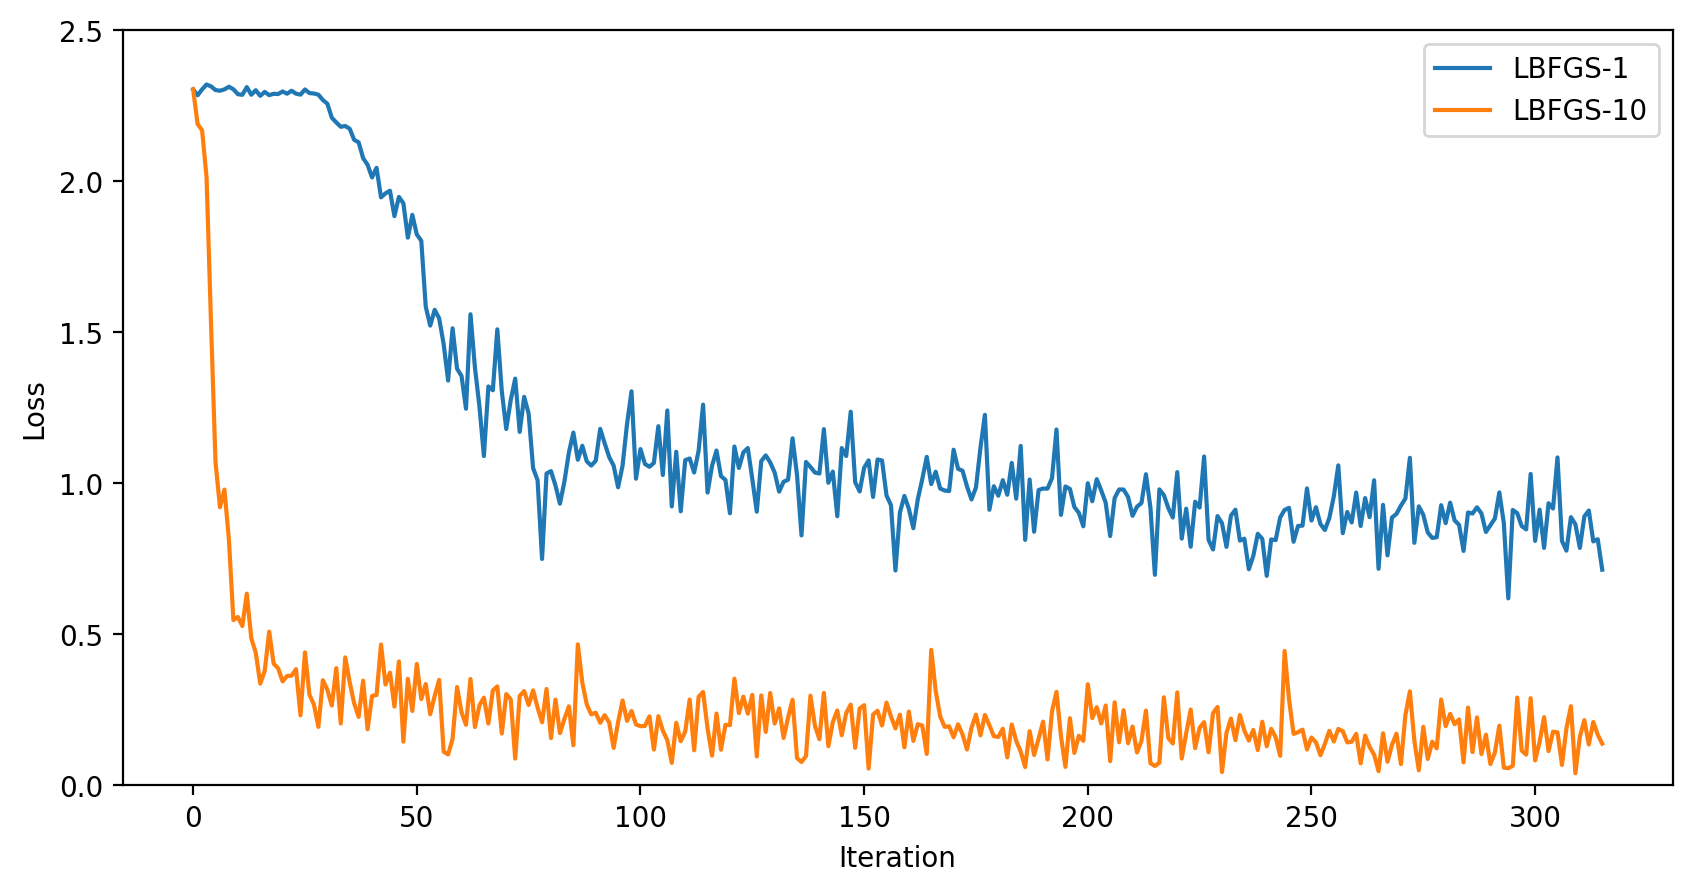
\includegraphics[width=0.9\linewidth]{fig-mnist-limit-lbfgs.png}
    \caption{L-BFGS算法在不允许内部更新时的训练结果}
    \label{fig:mnist_limit_lbfgs}
\end{figure}

图\ref{fig:mnist_train}中,L-BFGS算法看似获得了最快的优化速度,但这需要每轮在相同输入下进行十轮内部更新,这导致优化相同的总轮数时,L-BFGS算法消耗的时间大约为其他算法的两倍。如果不允许内部更新,L-BFGS算法消耗的时间与其他算法接近,但是优化结果会明显变差,如图\ref{fig:mnist_limit_lbfgs}所示,LGBFS-1曲线代表了不允许内部多次更新的情况。

\section{总结}

本文尝试使用L-BFGS算法对神经网络进行训练,通过与随机梯度下降和Adam算法进行对比,分析了L-BFGS算法的优势和劣势。L-BFGS算法在优化目标固定的情况下,能够获得较快的收敛速度,但是在优化目标随时变化的情况下,L-BFGS算法的收敛速度较慢,甚至无法收敛。

此外,相较于Adam算法,L-BFGS算法依然更复杂,所需要的计算开销也更大。同时,现在的深度学习领域有数据集规模越来越大的趋势,研究人员更倾向于让模型在更多的数据上训练,而不是对少量数据获得更好的拟合,如果过于关注对部分数据的拟合,反而可能让模型产生过拟合。基于一阶梯度的优化方法可以给模型提供更多的“探索”机会,从而获得更好的泛化能力。当前,Adam算法已经可以满足绝大多数深度学习任务的训练需求,当前的研究重点更多放在如何设计更好的网络结构上。

综上所述,L-BFGS算法是一种优秀的优化问题求解算法,但是在实际的深度学习领域,它的应用场景较为有限。

\section*{附:代码}

\subsection*{lbfgs.py}
\begin{lstlisting}[language=python,numbers=left]
import torch
from collections import deque

class LBFGS():
    def __init__(self, params, lr = 0.01 , max_iter=100, 
            memory_size=10, line_search_fn=None):
        self.max_iter = max_iter
        self.memory_size = memory_size
        self.line_search_fn = line_search_fn
        self.s = deque(maxlen=memory_size)
        self.y = deque(maxlen=memory_size)
        self.rho = deque(maxlen=memory_size)
        self._params = list(params)
        self.last_s = None
        self.last_grad = None
        self.lr = lr
    
    def update_memory(self, s, y):
        ys = torch.dot(y, s)
        if ys > 1e-10:
            self.s.append(s)
            self.y.append(y)
            self.rho.append(1. / ys)
    
    @torch.no_grad()
    def compute_direction(self, grad):
        y = self.y[-1]
        s = self.s[-1]
        ys = torch.dot(y, s)
        q = grad.clone()
        alpha = []
        for s, y, rho in zip(reversed(self.s), reversed(self.y), reversed(self.rho)):
            alpha_i = rho * torch.dot(s, q)
            q.add_(y, alpha=-alpha_i)
            alpha.append(alpha_i)

        H_diag = ys / y.dot(y)
        r = torch.mul(q, H_diag)
        for s, y, rho, alpha_i in zip(self.s, self.y, self.rho, reversed(alpha)):
            beta = rho * torch.dot(y, r)
            r.add_(s, alpha=alpha_i - beta)
        return -r
    
    def zero_grad(self):
        for p in self._params:
            if p.grad is not None:
                p.grad.detach_()
                p.grad.zero_()

    def _gather_flat_grad(self):
        views = []
        for p in self._params:
            if p.grad is None:
                view = p.new(p.numel()).zero_()
            elif p.grad.is_sparse:
                view = p.grad.to_dense().view(-1)
            else:
                view = p.grad.view(-1)
            views.append(view)
        return torch.cat(views, 0)
    
    def _add_grad(self, step_size, update):
        offset = 0
        for p in self._params:
            numel = p.numel()
            p.add_(update[offset:offset + numel].view_as(p), alpha=step_size)
            offset += numel
        assert offset == self._gather_flat_grad().numel()

    @torch.no_grad()
    def step(self, closure = None):
        loss = None
        if closure is not None:
            closure = torch.enable_grad()(closure)
            loss = closure()
            loss = loss.item()
        grad = self._gather_flat_grad()
        if grad is None:
            raise ValueError("Function must compute gradients.")
        if self.last_grad is not None and self.last_s is not None:
            self.update_memory(self.last_s, grad - self.last_grad)
            self.last_grad = None
            self.last_s = None
        if len(self.s) > 0:
            p = self.compute_direction(grad)
        else:
            p = -grad
        alpha = self.lr
        s = alpha * p
        self._add_grad(alpha, p)
        
        self.last_s = s
        self.last_grad = grad.clone()

        return loss
\end{lstlisting}


\subsection*{train.py}
\begin{lstlisting}[language=python,numbers=left]
import torch
from torchvision import datasets, transforms
import torch.nn as nn
import numpy as np
from lbfgs import LBFGS

class SimpleCNN(nn.Module):
    def __init__(self):
        super(SimpleCNN, self).__init__()
        self.conv1 = nn.Conv2d(1, 16, kernel_size=3, stride=1, padding=1)
        self.relu1 = nn.ReLU()
        self.pool1 = nn.MaxPool2d(kernel_size=2, stride=2)
        self.conv2 = nn.Conv2d(16, 32, kernel_size=3, stride=1, padding=1)
        self.relu2 = nn.ReLU()
        self.pool2 = nn.MaxPool2d(kernel_size=2, stride=2)
        self.fc1 = nn.Linear(7 * 7 * 32, 128)
        self.relu3 = nn.ReLU()
        self.fc2 = nn.Linear(128, 10)

    def forward(self, x):
        x = self.conv1(x)
        x = self.relu1(x)
        x = self.pool1(x)
        x = self.conv2(x)
        x = self.relu2(x)
        x = self.pool2(x)
        x = x.view(-1, 7 * 7 * 32)
        x = self.fc1(x)
        x = self.relu3(x)
        x = self.fc2(x)
        return x


root = "~/data/MNIST"

# load the dataset and pre-process
transform=transforms.Compose([
    transforms.ToTensor(),
    transforms.Normalize((0.1307,), (0.3081,))
    ])
train_dataset = datasets.MNIST(root, train=True, transform=transform)


model = SimpleCNN()
model.cuda()
dataloader = torch.utils.data.DataLoader(train_dataset, batch_size=128)
criterion = nn.CrossEntropyLoss()
optimizer = LBFGS(model.parameters(), lr=0.01)
loss_list = []
for epoch in range(4):
    for batch_idx, (x, target) in enumerate(dataloader):
        x = x.cuda()
        target = target.cuda()
        def closure():
            optimizer.zero_grad()
            output = model(x)
            loss = criterion(output, target)
            loss.backward()
            return loss
        for i in range(10):
            loss = optimizer.step(closure)
            loss_list.append(loss)
\end{lstlisting}


\end{document}
